% The generic preamble
\documentclass[10pt,letterpaper,fleqn,titlepage]{article}

% Define packages to use
\usepackage{natbib}
\usepackage[dvips]{graphicx,color}
\usepackage{amsmath,amssymb}
\usepackage{bm}
\usepackage{caption}
\usepackage{xr}
\usepackage{ifthen}
\usepackage[dvipdfm,colorlinks,linkcolor=blue,citecolor=blue,urlcolor=blue]{hyperref}
\usepackage{fancybox}
\usepackage{textcomp}
\usepackage{alltt}
%\usepackage{floatflt}
%\usepackage{svn}


% Redefine default page
\setlength{\textheight}{9in}  % 1" above and below
\setlength{\textwidth}{6.75in}   % 0.5" left and right
\setlength{\oddsidemargin}{-0.25in}

% Redefine default paragraph
\setlength{\parindent}{0pt}
\setlength{\parskip}{1ex plus 0.5ex minus 0.2ex}

% Define caption width and default fonts
\setlength{\captionmargin}{0.5in}
\renewcommand{\captionfont}{\sffamily}
\renewcommand{\captionlabelfont}{\bfseries\sffamily}

% Define commands for super- and subscript in text mode
\newcommand{\superscript}[1]{\ensuremath{^\textrm{#1}}}
\newcommand{\subscript}[1]{\ensuremath{_\textrm{#1}}}

% Derived commands
\newcommand{\invcm}{\textrm{cm\superscript{-1}}}
\newcommand{\micron}{\ensuremath{\mu\textrm{m}}}

\newcommand{\df}{\ensuremath{\delta f}}
\newcommand{\Df}{\ensuremath{\Delta f}}
\newcommand{\dx}{\ensuremath{\delta x}}
\newcommand{\Dx}{\ensuremath{X_{max}}}
\newcommand{\Xeff}{\ensuremath{X_{eff}}}

\newcommand{\water}{\textrm{H\subscript{2}O}}
\newcommand{\carbondioxide}{\textrm{CO\subscript{2}}}
\newcommand{\ozone}{\textrm{O\subscript{3}}}

\newcommand{\taup}[1]{\ensuremath{\tau_{#1}}}
\newcommand{\efftaup}[1]{\ensuremath{\tau_{#1}^{*}}}

\newcommand{\textbfm}[1]{\boldmath\ensuremath{#1}\unboldmath}

\newcommand{\rb}[1]{\raisebox{1.5ex}[0pt]{#1}}

\newcommand{\f}[1]{\texttt{#1}}

% Define how equations are numbered
\numberwithin{equation}{section}
\numberwithin{figure}{section}
\numberwithin{table}{section}

% Define a command for title page author email footnote
\newcommand{\email}[1]
{%
  \renewcommand{\thefootnote}{\alph{footnote}}%
  \footnote{#1}
  \renewcommand{\thefootnote}{\arabic{footnote}}
}

% Define a command to print the Office Note subheading
\newcommand{\notesubheading}[1]
{%
  \ifthenelse{\equal{#1}{}}{}
  { {\Large\bfseries Office Note #1\par}%
    {\scriptsize \sc This is an unreviewed manuscript, primarily intended for informal}\\ 
    {\scriptsize \sc exchange of information among JCSDA researchers\par}%
  }
}

% Redefine the maketitle macro
\makeatletter
\def\docseries#1{\def\@docseries{#1}}
\def\docnumber#1{\def\@docnumber{#1}}
\renewcommand{\maketitle}
{%
  \thispagestyle{empty}
  \vspace*{1in}
  \begin{center}%
     \sffamily
     {\huge\bfseries Joint Center for Satellite Data Assimilation\par}%
     \notesubheading{\@docnumber}
  \end{center}
  \begin{flushleft}%
     \sffamily
     \vspace*{0.5in}
     {\Large\bfseries\ifthenelse{\equal{\@docseries}{}}{}{\@docseries: }\@title\par}%
     \medskip
     {\large\@author\par}%
     \medskip
     {\large\@date\par}%
     \bigskip\hrule\vspace*{2pc}%
  \end{flushleft}%
  \newpage
  \setcounter{footnote}{0}
}
\makeatother
\docseries{}
\docnumber{}


% Define a command for a DRAFT watermark
\usepackage{eso-pic}
\newcommand{\draftwatermark}
{
  \AddToShipoutPicture{%
    \definecolor{lightgray}{gray}{.85}
    \setlength{\unitlength}{1in}
    \put(2.5,3.5){%
      \rotatebox{45}{%
        \resizebox{4in}{1in}{%
          \textsf{\textcolor{lightgray}{DRAFT}}
        }
      }
    }
  }
}




% Include files
\includeonly{Imager_SRF_Data_Plots.app,Sounder_SRF_Data_Plots.app,Imager_Tfit_Data_Plots.app,Sounder_Tfit_Data_Plots.app}

% Subversion keywords
\SVN $Date$
\SVN $Revision$

% Title info
\title{INSAT-3D Imager and Sounder Spectral Response Function Processing}
\author{Paul van Delst\email{paul.vandelst@noaa.gov}\\NCEP/EMC/IMSG}
\date{\SVNDate ; rev\SVNRevision}
\docnumber{3}
\docseries{CRTM}


%-------------------------------------------------------------------------------
%                            Ze document begins...
%-------------------------------------------------------------------------------
\begin{document}
\maketitle

%\draftwatermark

% The front matter
%=================
\thispagestyle{empty}
\vspace*{10cm}
\begin{center}
  {\sffamily\Large\bfseries Change History}
  \begin{table}[htp]
    \centering
    \begin{tabular}{|p{2cm}|p{3cm}|p{8cm}|}
      \hline
      \sffamily\textbf{Date} & \sffamily\textbf{Author} & \sffamily\textbf{Change}\\
      \hline\hline
      2013-11-21 & Paul van Delst & Initial draft.\\
      \hline
      2014-07-07 & Paul van Delst & Modified for updated SRF data.\\
      \hline
    \end{tabular}
  \end{table}
\end{center}
\clearpage
\pagestyle{fancy}
\fancyhead[LE,RO]{\sffamily \rightmark}
\fancyhead[LO,RE]{\sffamily \leftmark}
\pagenumbering{arabic}
\setcounter{page}{1}


% The main matter
%================

\section{Introduction}
%=====================
This document describes the pre-processing applied to the INSAT-3D Imager and Sounder instruments updated spectral response functions (SRFs), obtained from \cite{INSAT3D_SRF_Data2} in June 2014, to prepare for use in the CRTM processing chain. The SRFs are used to generate channel central frequencies, as well as in the convolution of monochromatic quantities such as Planck radiances or line-by-line (LBL) model generated transmittances to produce such things as polychromatic correction coefficients and instrument resolution transmittances. The latter, for a diverse set of atmospheric profiles, are then regressed against a set of predictors to produce the fast transmittance model coefficients used by the CRTM.

Comparisons are also made with the original SRF dataset \citep{INSAT3D_SRF_Data} obtained in October 2013.


\subsection{Computation of the channel central frequency}
%--------------------------------------------------------
The computed imager and sounder channel central frequencies, $\nu_0$, are the first moments of the defined SRF, $\phi(\nu)$,
\begin{equation}
  \nu_0 = \frac{\displaystyle\int{\nu\:\phi(\nu)\ud \nu}}{\displaystyle\int{\phi(\nu)\ud \nu}}
\end{equation}


\subsection{Computation of polychromatic correction coefficients}
%----------------------------------------------------------------
In the CRTM, the conversion of \emph{channel resolution} radiances to brightness temperatures has to take the channel bandwidth into account. For any channel, the regression relation to be solved is

\begin{equation}
  a_0 + a_1T + \ldots = \frac{\displaystyle k_1}{\displaystyle \ln\left[\frac{k_2}{R(T)}+1\right]} = Y(T)
  \label{eqn:polycorr_regression}
\end{equation}
where
\begin{equation*}
  \begin{array}{r@{\;=\;}l}
         T &\mbox{brightness temperature} \\
        a_j&\mbox{regression coefficients} \\
    k_1,k_2&\mbox{Planck coefficients} \\
       R(T)&\mbox{channel radiance} \\
       Y(T)&\mbox{``effective'' brightness temperature, or $T_{eff}$}
  \end{array}
\end{equation*}
and the channel radiances used to determine the effective temperatures, $Y(T)$, are computed the usual way
\begin{equation}
  R(T) = \frac{\displaystyle\int{B(T,\nu)\:\phi(\nu)\ud \nu}}{\displaystyle\int{\phi(\nu)\ud \nu}}
\end{equation}
The quantity minimised to obtain the $a_j$ coefficients is
\begin{equation}
  \left[ \sum_{j=0}^{M}a_j T_{i} - Y(T_{i}) \right]^2 \quad\mbox{for}\quad T_i = 150K, \ldots, 340K \;\mbox{ in 5K steps.}
\end{equation}
Currently the number of coefficients is fixed at two (i.e. $M=1$).



\newpage
\section{Summary}
%================

The following tables list the computed central frequencies and polychromatic correction coefficients for the imager and sounder instruments, as well the differences with the same quantities obtained from the original set of SRFs.

\subsection{Imager}
%------------------

Plots of the Imager SRF data, and their differences, are shown in appendix \ref{app.imgr_srf_data_plots}. The temperature fit residuals for each channel, and their differences from those of the original SRF dataset, are shown in appendix \ref{app.imgr_tfit_data_plots}.

\begin{table}[htp]
  \centering
  \begin{tabular}{C{1.5cm} R{1.5cm}@{.}L{1.5cm} *{2}{R{1cm}@{.}L{2cm}}}
    \hline
    \sffamily{Imager} & \multicolumn{2}{c}{$\nu_0$} & \multicolumn{2}{c}{$a_0$ \textsf{(offset)}} & \multicolumn{2}{c}{$a_1$ \textsf{(slope)}} \\
    \sffamily{Channel} & \multicolumn{2}{c}{\sffamily{(\invcm)}} & \multicolumn{2}{c}{\sffamily{(K)}} & \multicolumn{2}{c}{\sffamily{(K/K)}}  \\
    \hline\hline
    3  & 2548&42014 & 0&39830363 & 0&99942687 \\
    4  & 1454&40973 & 0&62372841 & 0&99852040 \\
    5  &  925&09803 & 0&38137920 & 0&99868532 \\
    6  &  837&38593 & 0&26594109 & 0&99899992 \\
    \hline
  \end{tabular}
  \caption{The computed INSAT-3D Imager channel central frequencies and polychromatic correction coefficients.}
  \label{tab:imgr_insat3d_results}
\end{table}


\begin{table}[htp]
  \centering
  \begin{tabular}{C{1.5cm} *{3}{R{1cm}@{.}L{2cm}}}
    \hline
    \sffamily{Imager} & \multicolumn{2}{c}{$\Delta \nu_0$} & \multicolumn{2}{c}{$\Delta a_0$ \textsf{(offset)}} & \multicolumn{2}{c}{$\Delta a_1$ \textsf{(slope)}} \\
    \sffamily{Channel} & \multicolumn{2}{c}{\sffamily{(\invcm)}} & \multicolumn{2}{c}{\sffamily{(K)}} & \multicolumn{2}{c}{\sffamily{(K/K)}}  \\
    \hline\hline
    3  &  1&222473e-01 &  5&340637e-03 & -7&614884e-06 \\
    4  & -2&330886e-01 & -5&954575e-03 &  1&229867e-05 \\
    5  &  2&532271e-01 &  9&930551e-04 & -3&163284e-06 \\
    6  &  5&192023e-01 &  1&575004e-03 & -5&534034e-06 \\
    \hline
  \end{tabular}
  \caption{The difference between the computed INSAT-3D Imager channel central frequencies and polychromatic correction coefficients for the updated SRFs.}
  \label{tab:imgr_insat3d_results_difference}
\end{table}



\subsection{Sounder}
%-------------------

Plots of the Sounder SRF data, and their differences, are shown in appendix \ref{app.sndr_srf_data_plots}. The temperature fit residuals for each channel, and their differences from those of the original SRF dataset, are shown in appendix \ref{app.sndr_tfit_data_plots}.

It should be noted here that there are significant SRF differences for some of the sounder channels, in particular the shortware channels 13-18. For these channels there is a sgnificant shift of the SRFs to lower frequencies. This is reflected in the central frequency differences shown in table \ref{tab:sndr_insat3d_results_difference}, with $\Delta \nu_0$ values for channels 13-18 ranging from 7-15\invcm. See figures \ref{fig:sndr_ch13} to \ref{fig:sndr_ch18} for plots of those particular SRFs.

\begin{table}[htp]
  \centering
  \begin{tabular}{C{1.5cm} R{1.5cm}@{.}L{1.5cm} *{2}{R{1cm}@{.}L{2cm}}}
    \hline
    \sffamily{Sounder} & \multicolumn{2}{c}{$\nu_0$} & \multicolumn{2}{c}{$a_0$ \textsf{(offset)}} & \multicolumn{2}{c}{$a_1$ \textsf{(slope)}} \\
    \sffamily{Channel} & \multicolumn{2}{c}{\sffamily{(\invcm)}} & \multicolumn{2}{c}{\sffamily{(K)}} & \multicolumn{2}{c}{\sffamily{(K/K)}}  \\
    \hline\hline
    1 &  681&62206 & 0&03046981 & 0&99986043 \\
    2 &  698&62139 & 0&01879741 & 0&99991614 \\
    3 &  712&58032 & 0&02289618 & 0&99989992 \\
    4 &  733&35257 & 0&03227880 & 0&99986293 \\
    5 &  750&09886 & 0&03643214 & 0&99984866 \\
    6 &  794&15150 & 0&09316524 & 0&99963313 \\
    7 &  834&32264 & 0&19522736 & 0&99926418 \\
    8 &  909&58337 & 0&17639610 & 0&99938313 \\
    9 & 1031&98619 & 0&06386464 & 0&99979895 \\
   10 & 1346&10910 & 0&18572004 & 0&99952975 \\
   11 & 1420&56284 & 0&39893243 & 0&99903751 \\
   12 & 1533&28319 & 0&23487739 & 0&99946755 \\
   13 & 2167&56741 & 0&03284663 & 0&99994502 \\
   14 & 2202&05890 & 0&03255260 & 0&99994615 \\
   15 & 2232&00124 & 0&03692231 & 0&99993955 \\
   16 & 2407&95850 & 0&06765204 & 0&99989696 \\
   17 & 2495&40576 & 0&07411556 & 0&99989035 \\
   18 & 2642&07962 & 0&29912655 & 0&99958143 \\
    \hline
  \end{tabular}
  \caption{The computed INSAT-3D Sounder channel central frequencies and polychromatic correction coefficients.}
  \label{tab:sndr_insat3d_results}
\end{table}

\begin{table}[htp]
  \centering
  \begin{tabular}{C{1.5cm} *{3}{R{1cm}@{.}L{2cm}}}
    \hline
    \sffamily{Sounder} & \multicolumn{2}{c}{$\Delta \nu_0$} & \multicolumn{2}{c}{$\Delta a_0$ \textsf{(offset)}} & \multicolumn{2}{c}{$\Delta a_1$ \textsf{(slope)}} \\
    \sffamily{Channel} & \multicolumn{2}{c}{\sffamily{(\invcm)}} & \multicolumn{2}{c}{\sffamily{(K)}} & \multicolumn{2}{c}{\sffamily{(K/K)}}  \\
    \hline\hline
    1 & -2&384271e-02 & -3&624546e-03 &  1&668416e-05 \\
    2 &  8&865027e-02 & -1&526845e-02 &  6&818310e-05 \\
    3 &  4&900753e-01 & -4&772684e-03 &  2&092925e-05 \\
    4 &  3&295078e-01 & -8&518261e-03 &  3&620886e-05 \\
    5 & -6&201422e-01 & -5&343381e-03 &  2&205690e-05 \\
    6 &  1&554839e+00 & -6&541811e-03 &  2&635550e-05 \\
    7 &  7&305848e-02 & -6&097686e-03 &  2&316287e-05 \\
    8 &  3&525065e+00 &  3&889811e-03 & -1&204881e-05 \\
    9 &  2&663744e+00 &  7&985571e-03 & -2&478078e-05 \\
   10 &  1&640695e+00 & -4&912065e-02 &  1&249970e-04 \\
   11 & -1&523594e+00 & -1&921560e-01 &  4&823958e-04 \\
   12 &  2&733226e+00 & -1&121861e-01 &  2&577023e-04 \\
   13 & -1&597081e+01 &  9&645771e-04 & -1&859146e-06 \\
   14 & -7&024429e+00 &  7&376784e-04 & -1&467514e-06 \\
   15 & -9&069491e+00 & -1&235584e-03 &  1&723795e-06 \\
   16 & -1&180761e+01 &  2&795438e-03 & -4&620730e-06 \\
   17 & -1&464507e+01 &  5&941099e-04 & -1&262977e-06 \\
   18 & -1&554782e+01 &  2&980200e-02 & -4&402094e-05 \\
    \hline
  \end{tabular}
  \caption{The difference between the computed INSAT-3D Sounder channel central frequencies and polychromatic correction coefficients for the updated SRFs.}
  \label{tab:sndr_insat3d_results_difference}
\end{table}


\newpage
\section{Truncation of SRF data}
%===============================
\label{sec:data_truncation}

The SRFs were reported on the same frequency grid for all channels in an instrument, with out-of-band responses set to zero. To minimise the number of frequencies for which LBL calculations would be done, the SRF data were truncated to eliminate the zero-valued out-of-band elements. The truncation points were selected automatically by determining the first non-zero point either side of the SRF, and then extending back 20 data points.

\subsection{Imager}
%------------------
The truncation frequencies for the imager instrument are shown in table \ref{tab:imgr_insat3d_truncation}. The ``character'' of the imager SRFs at low response levels near the truncations points are shown in figure \ref{fig:imgr_ch3-6_trunc}


\begin{table}[htp]
  \centering
  \begin{tabular}{c *{2}{c r@{.}l}}
    \hline
    \sffamily{Sounder} & & \multicolumn{2}{c}{$\nu_1$} & & \multicolumn{2}{c}{$\nu_2$}  \\
    \sffamily{Channel} & & \multicolumn{2}{c}{\sffamily{(\invcm)}} & & \multicolumn{2}{c}{\sffamily{(\invcm)}} \\
    \hline\hline
    3 & & 2449&10 & & 2647&40  \\
    4 & & 1338&60 & & 1564&40  \\
    5 & &  869&20 & &  986&20  \\
    6 & &  788&00 & &  882&20  \\
    \hline
  \end{tabular}
  \caption{The frequencies at which the INSAT-3D Imager channel SRFs were truncated prior to processing.}
  \label{tab:imgr_insat3d_truncation}
\end{table}

\begin{figure}[H]
  \centering
  \begin{tabular}{c c}
    \includegraphics[scale=0.35]{graphics/imgr/trunc/imgr_insat3d-3.trunc.eps} &
    \includegraphics[scale=0.35]{graphics/imgr/trunc/imgr_insat3d-4.trunc.eps} \\
    \includegraphics[scale=0.35]{graphics/imgr/trunc/imgr_insat3d-5.trunc.eps} &
    \includegraphics[scale=0.35]{graphics/imgr/trunc/imgr_insat3d-6.trunc.eps}
  \end{tabular}
  \caption{INSAT-3D Imager channels 3-6 SRFs at low response levels near the truncation frequencies.}
  \label{fig:imgr_ch3-6_trunc}
\end{figure}


\subsection{Sounder}
%-------------------
The truncation frequencies for the sounder instrument are shown in table \ref{tab:sndr_insat3d_truncation}. The ``character'' of the sounder SRFs, for a selection of channels, at low response levels near the truncations points are shown in figure \ref{fig:sndr_selection_trunc}. 



\begin{table}[htp]
  \centering
  \begin{tabular}{c *{2}{c r@{.}l}}
    \hline
    \sffamily{Sounder} & & \multicolumn{2}{c}{$\nu_1$} & & \multicolumn{2}{c}{$\nu_2$}  \\
    \sffamily{Channel} & & \multicolumn{2}{c}{\sffamily{(\invcm)}} & & \multicolumn{2}{c}{\sffamily{(\invcm)}} \\
    \hline\hline
     1 & &   660&90 & &  704&70 \\
     2 & &   683&30 & &  715&20 \\
     3 & &   695&50 & &  730&00 \\
     4 & &   712&70 & &  757&30 \\
     5 & &   727&50 & &  776&60 \\
     6 & &   758&30 & &  831&60 \\
     7 & &   781&50 & &  884&30 \\
     8 & &   861&20 & &  962&80 \\
     9 & &   996&90 & & 1068&90 \\
    10 & &  1271&50 & & 1409&20 \\
    11 & &  1319&40 & & 1524&90 \\
    12 & &  1458&30 & & 1605&50 \\
    13 & &  2135&20 & & 2208&10 \\
    14 & &  2168&50 & & 2237&70 \\
    15 & &  2197&20 & & 2268&10 \\
    16 & &  2363&60 & & 2457&40 \\
    17 & &  2447&00 & & 2547&40 \\
    18 & &  2552&00 & & 2736&80 \\
    \hline
  \end{tabular}
  \caption{The frequencies at which the INSAT-3D Sounder channel SRFs were truncated prior to processing.}
  \label{tab:sndr_insat3d_truncation}
\end{table}

\begin{figure}[H]
  \centering
  \begin{tabular}{c c}
    \includegraphics[scale=0.35]{graphics/sndr/trunc/sndr_insat3d-1.trunc.eps} &
    \includegraphics[scale=0.35]{graphics/sndr/trunc/sndr_insat3d-6.trunc.eps} \\
    \includegraphics[scale=0.35]{graphics/sndr/trunc/sndr_insat3d-8.trunc.eps} &
    \includegraphics[scale=0.35]{graphics/sndr/trunc/sndr_insat3d-10.trunc.eps}
  \end{tabular}
  \caption{A selection of INSAT-3D Sounder channel SRFs at low response levels near the trunction frequencies.}
  \label{fig:sndr_selection_trunc}
\end{figure}


\newpage
\section{Impact of updated SRFs on convolved radiances}
%======================================================
\label{sec:updated_impact}
To determine the impact of the updated SRFs on the convolved channel radiancesd, both sets of data (original and updated SRFs) were convolved with LBL-model generated radiances.

LBLRTM \citep{Clough_2005} v12.2 was used with the ECMWF83 atmospheric profile dataset to generate radiance spectra. The radiance spectra were convovled with the SRFs to yield channel resolution radiances which were then converted to brightness temperatures for each SRF set. The statistics of the brightness temperature differences for the Imager instrument are shown in figure \ref{fig:imgr_dTb_stats}, and in \ref{fig:sndr_dTb_stats} for the Sounder. For the Imager, the largest individual differences are the hundredths of a Kelvin level. For the Sounder, however, the large differences between the original and updated SRF datasets for the shortwave channels, 13-18 (see figures \ref{fig:sndr_ch13}-\ref{fig:sndr_ch18}), are reflected in the 4-8K brightness temperatures differences for some of those channels, 13-16. Channels 17 and 18 are less affected by the SRF shifts as they are window channels.

\begin{figure}[H]
  \centering
  \includegraphics[scale=0.8]{graphics/imgr/imgr_insat3d.dTb_stats.eps}
  \caption{Statistics of the brightness temperature differences between the original and updated INSAT-3D Imager SRFs. The calculations used LBLRTM v12.2 and the ECMWF83 profile dataset with a surface emissivity of 0.95.}
  \label{fig:imgr_dTb_stats}
\end{figure}

\begin{figure}[H]
  \centering
  \includegraphics[scale=0.8]{graphics/sndr/sndr_insat3d.dTb_stats.eps}
  \caption{Statistics of the brightness temperature differences between the original and updated INSAT-3D Sounder SRFs. The calculations used LBLRTM v12.2 and the ECMWF83 profile dataset with a surface emissivity of 0.95.}
  \label{fig:sndr_dTb_stats}
\end{figure}

% The references section
%=======================
\clearpage
\bibliographystyle{plainnat}
\bibliography{bibliography}


% The appendices section
%=======================
\begin{appendix}
  \phantomsection
\section{INSAT-3D Imager SRF Data Plots}
%=======================================
\label{app.imgr_srf_data_plots}

\begin{figure}[H]
  \centering
  \begin{tabular}{c}
    \includegraphics[scale=0.55]{graphics/imgr/srf/imgr_insat3d-3.eps} \\
    \includegraphics[scale=0.55]{graphics/imgr/srf/imgr_insat3d-3.difference.eps}
  \end{tabular}
  \caption{INSAT-3D Imager channel 3 spectral responses. Vertical dashed lines are the locations of the computed central frequencies. \emph{(Top)} Comparison of original and new SRFs. \emph{(Bottom)} Response difference between the original and new SRFs.}
  \label{fig:imgr_ch3}
\end{figure}


\begin{figure}[H]
  \centering
  \begin{tabular}{c}
    \includegraphics[scale=0.55]{graphics/imgr/srf/imgr_insat3d-4.eps} \\
    \includegraphics[scale=0.55]{graphics/imgr/srf/imgr_insat3d-4.difference.eps}
  \end{tabular}
  \caption{INSAT-3D Imager channel 4 spectral responses. Vertical dashed lines are the locations of the computed central frequencies. \emph{(Top)} Comparison of original and new SRFs. \emph{(Bottom)} Response difference between the original and new SRFs.}
  \label{fig:imgr_ch4}
\end{figure}


\begin{figure}[H]
  \centering
  \begin{tabular}{c}
    \includegraphics[scale=0.55]{graphics/imgr/srf/imgr_insat3d-5.eps} \\
    \includegraphics[scale=0.55]{graphics/imgr/srf/imgr_insat3d-5.difference.eps}
  \end{tabular}
  \caption{INSAT-3D Imager channel 5 spectral responses. Vertical dashed lines are the locations of the computed central frequencies. \emph{(Top)} Comparison of original and new SRFs. \emph{(Bottom)} Response difference between the original and new SRFs.}
  \label{fig:imgr_ch5}
\end{figure}


\begin{figure}[H]
  \centering
  \begin{tabular}{c}
    \includegraphics[scale=0.55]{graphics/imgr/srf/imgr_insat3d-6.eps} \\
    \includegraphics[scale=0.55]{graphics/imgr/srf/imgr_insat3d-6.difference.eps}
  \end{tabular}
  \caption{INSAT-3D Imager channel 6 spectral responses. Vertical dashed lines are the locations of the computed central frequencies. \emph{(Top)} Comparison of original and new SRFs. \emph{(Bottom)} Response difference between the original and new SRFs.}
  \label{fig:imgr_ch6}
\end{figure}

  \section{INSAT-3D Imager Polychromatic Correction Temperature Fit Residual Data Plots}
%=====================================================================================
\label{app.imgr_tfit_data_plots}
%\newpage

\begin{figure}[H]
  \centering
  \begin{tabular}{c}
    \includegraphics[scale=0.55]{graphics/imgr/tfit/imgr_insat3d-3.tfit.eps} \\
    \includegraphics[scale=0.55]{graphics/imgr/tfit/imgr_insat3d-3.tfit.difference.eps}
  \end{tabular}
  \caption{INSAT-3D Imager channel 3 polychromatic correction temperature fit residuals. \emph{(Top)} Comparison of residuals for original and new SRFs. \emph{(Bottom)} Residual differences for the original and new SRFs.}
  \label{fig:imgr_ch3_tfit}
\end{figure}


\begin{figure}[H]
  \centering
  \begin{tabular}{c}
    \includegraphics[scale=0.55]{graphics/imgr/tfit/imgr_insat3d-4.tfit.eps} \\
    \includegraphics[scale=0.55]{graphics/imgr/tfit/imgr_insat3d-4.tfit.difference.eps}
  \end{tabular}
  \caption{INSAT-3D Imager channel 4 polychromatic correction temperature fit residuals. \emph{(Top)} Comparison of residuals for original and new SRFs. \emph{(Bottom)} Residual differences for the original and new SRFs.}
  \label{fig:imgr_ch4_tfit}
\end{figure}


\begin{figure}[H]
  \centering
  \begin{tabular}{c}
    \includegraphics[scale=0.55]{graphics/imgr/tfit/imgr_insat3d-5.tfit.eps} \\
    \includegraphics[scale=0.55]{graphics/imgr/tfit/imgr_insat3d-5.tfit.difference.eps}
  \end{tabular}
  \caption{INSAT-3D Imager channel 5 polychromatic correction temperature fit residuals. \emph{(Top)} Comparison of residuals for original and new SRFs. \emph{(Bottom)} Residual differences for the original and new SRFs.}
  \label{fig:imgr_ch5_tfit}
\end{figure}


\begin{figure}[H]
  \centering
  \begin{tabular}{c}
    \includegraphics[scale=0.55]{graphics/imgr/tfit/imgr_insat3d-6.tfit.eps} \\
    \includegraphics[scale=0.55]{graphics/imgr/tfit/imgr_insat3d-6.tfit.difference.eps}
  \end{tabular}
  \caption{INSAT-3D Imager channel 6 polychromatic correction temperature fit residuals. \emph{(Top)} Comparison of residuals for original and new SRFs. \emph{(Bottom)} Residual differences for the original and new SRFs.}
  \label{fig:imgr_ch6_tfit}
\end{figure}



  \phantomsection
\section{INSAT-3D Sounder SRF Data Plots}
%========================================
\label{app.sndr_srf_data_plots}

\begin{figure}[H]
  \centering
  \begin{tabular}{c}
    \includegraphics[scale=0.55]{graphics/sndr/srf/sndr_insat3d-1.eps} \\
    \includegraphics[scale=0.55]{graphics/sndr/srf/sndr_insat3d-1.difference.eps}
  \end{tabular}
  \caption{INSAT-3D Sounder channel 1 spectral responses. Vertical dashed lines are the locations of the computed central frequencies. \emph{(Top)} Comparison of original and new SRFs. \emph{(Bottom)} Response difference between the original and new SRFs.}
  \label{fig:sndr_ch1}
\end{figure}


\begin{figure}[H]
  \centering
  \begin{tabular}{c}
    \includegraphics[scale=0.55]{graphics/sndr/srf/sndr_insat3d-2.eps} \\
    \includegraphics[scale=0.55]{graphics/sndr/srf/sndr_insat3d-2.difference.eps}
  \end{tabular}
  \caption{INSAT-3D Sounder channel 2 spectral responses. Vertical dashed lines are the locations of the computed central frequencies. \emph{(Top)} Comparison of original and new SRFs. \emph{(Bottom)} Response difference between the original and new SRFs.}
  \label{fig:sndr_ch2}
\end{figure}


\begin{figure}[H]
  \centering
  \begin{tabular}{c}
    \includegraphics[scale=0.55]{graphics/sndr/srf/sndr_insat3d-3.eps} \\
    \includegraphics[scale=0.55]{graphics/sndr/srf/sndr_insat3d-3.difference.eps}
  \end{tabular}
  \caption{INSAT-3D Sounder channel 3 spectral responses. Vertical dashed lines are the locations of the computed central frequencies. \emph{(Top)} Comparison of original and new SRFs. \emph{(Bottom)} Response difference between the original and new SRFs.}
  \label{fig:sndr_ch3}
\end{figure}


\begin{figure}[H]
  \centering
  \begin{tabular}{c}
    \includegraphics[scale=0.55]{graphics/sndr/srf/sndr_insat3d-4.eps} \\
    \includegraphics[scale=0.55]{graphics/sndr/srf/sndr_insat3d-4.difference.eps}
  \end{tabular}
  \caption{INSAT-3D Sounder channel 4 spectral responses. Vertical dashed lines are the locations of the computed central frequencies. \emph{(Top)} Comparison of original and new SRFs. \emph{(Bottom)} Response difference between the original and new SRFs.}
  \label{fig:sndr_ch4}
\end{figure}


\begin{figure}[H]
  \centering
  \begin{tabular}{c}
    \includegraphics[scale=0.55]{graphics/sndr/srf/sndr_insat3d-5.eps} \\
    \includegraphics[scale=0.55]{graphics/sndr/srf/sndr_insat3d-5.difference.eps}
  \end{tabular}
  \caption{INSAT-3D Sounder channel 5 spectral responses. Vertical dashed lines are the locations of the computed central frequencies. \emph{(Top)} Comparison of original and new SRFs. \emph{(Bottom)} Response difference between the original and new SRFs.}
  \label{fig:sndr_ch5}
\end{figure}


\begin{figure}[H]
  \centering
  \begin{tabular}{c}
    \includegraphics[scale=0.55]{graphics/sndr/srf/sndr_insat3d-6.eps} \\
    \includegraphics[scale=0.55]{graphics/sndr/srf/sndr_insat3d-6.difference.eps}
  \end{tabular}
  \caption{INSAT-3D Sounder channel 6 spectral responses. Vertical dashed lines are the locations of the computed central frequencies. \emph{(Top)} Comparison of original and new SRFs. \emph{(Bottom)} Response difference between the original and new SRFs.}
  \label{fig:sndr_ch6}
\end{figure}


\begin{figure}[H]
  \centering
  \begin{tabular}{c}
    \includegraphics[scale=0.55]{graphics/sndr/srf/sndr_insat3d-7.eps} \\
    \includegraphics[scale=0.55]{graphics/sndr/srf/sndr_insat3d-7.difference.eps}
  \end{tabular}
  \caption{INSAT-3D Sounder channel 7 spectral responses. Vertical dashed lines are the locations of the computed central frequencies. \emph{(Top)} Comparison of original and new SRFs. \emph{(Bottom)} Response difference between the original and new SRFs.}
  \label{fig:sndr_ch7}
\end{figure}


\begin{figure}[H]
  \centering
  \begin{tabular}{c}
    \includegraphics[scale=0.55]{graphics/sndr/srf/sndr_insat3d-8.eps} \\
    \includegraphics[scale=0.55]{graphics/sndr/srf/sndr_insat3d-8.difference.eps}
  \end{tabular}
  \caption{INSAT-3D Sounder channel 8 spectral responses. Vertical dashed lines are the locations of the computed central frequencies. \emph{(Top)} Comparison of original and new SRFs. \emph{(Bottom)} Response difference between the original and new SRFs.}
  \label{fig:sndr_ch8}
\end{figure}


\begin{figure}[H]
  \centering
  \begin{tabular}{c}
    \includegraphics[scale=0.55]{graphics/sndr/srf/sndr_insat3d-9.eps} \\
    \includegraphics[scale=0.55]{graphics/sndr/srf/sndr_insat3d-9.difference.eps}
  \end{tabular}
  \caption{INSAT-3D Sounder channel 9 spectral responses. Vertical dashed lines are the locations of the computed central frequencies. \emph{(Top)} Comparison of original and new SRFs. \emph{(Bottom)} Response difference between the original and new SRFs.}
  \label{fig:sndr_ch9}
\end{figure}


\begin{figure}[H]
  \centering
  \begin{tabular}{c}
    \includegraphics[scale=0.55]{graphics/sndr/srf/sndr_insat3d-10.eps} \\
    \includegraphics[scale=0.55]{graphics/sndr/srf/sndr_insat3d-10.difference.eps}
  \end{tabular}
  \caption{INSAT-3D Sounder channel 10 spectral responses. Vertical dashed lines are the locations of the computed central frequencies. \emph{(Top)} Comparison of original and new SRFs. \emph{(Bottom)} Response difference between the original and new SRFs.}
  \label{fig:sndr_ch10}
\end{figure}


\begin{figure}[H]
  \centering
  \begin{tabular}{c}
    \includegraphics[scale=0.55]{graphics/sndr/srf/sndr_insat3d-11.eps} \\
    \includegraphics[scale=0.55]{graphics/sndr/srf/sndr_insat3d-11.difference.eps}
  \end{tabular}
  \caption{INSAT-3D Sounder channel 11 spectral responses. Vertical dashed lines are the locations of the computed central frequencies. \emph{(Top)} Comparison of original and new SRFs. \emph{(Bottom)} Response difference between the original and new SRFs.}
  \label{fig:sndr_ch11}
\end{figure}


\begin{figure}[H]
  \centering
  \begin{tabular}{c}
    \includegraphics[scale=0.55]{graphics/sndr/srf/sndr_insat3d-12.eps} \\
    \includegraphics[scale=0.55]{graphics/sndr/srf/sndr_insat3d-12.difference.eps}
  \end{tabular}
  \caption{INSAT-3D Sounder channel 12 spectral responses. Vertical dashed lines are the locations of the computed central frequencies. \emph{(Top)} Comparison of original and new SRFs. \emph{(Bottom)} Response difference between the original and new SRFs.}
  \label{fig:sndr_ch12}
\end{figure}


\begin{figure}[H]
  \centering
  \begin{tabular}{c}
    \includegraphics[scale=0.55]{graphics/sndr/srf/sndr_insat3d-13.eps} \\
    \includegraphics[scale=0.55]{graphics/sndr/srf/sndr_insat3d-13.difference.eps}
  \end{tabular}
  \caption{INSAT-3D Sounder channel 13 spectral responses. Vertical dashed lines are the locations of the computed central frequencies. \emph{(Top)} Comparison of original and new SRFs. \emph{(Bottom)} Response difference between the original and new SRFs.}
  \label{fig:sndr_ch13}
\end{figure}


\begin{figure}[H]
  \centering
  \begin{tabular}{c}
    \includegraphics[scale=0.55]{graphics/sndr/srf/sndr_insat3d-14.eps} \\
    \includegraphics[scale=0.55]{graphics/sndr/srf/sndr_insat3d-14.difference.eps}
  \end{tabular}
  \caption{INSAT-3D Sounder channel 14 spectral responses. Vertical dashed lines are the locations of the computed central frequencies. \emph{(Top)} Comparison of original and new SRFs. \emph{(Bottom)} Response difference between the original and new SRFs.}
  \label{fig:sndr_ch14}
\end{figure}


\begin{figure}[H]
  \centering
  \begin{tabular}{c}
    \includegraphics[scale=0.55]{graphics/sndr/srf/sndr_insat3d-15.eps} \\
    \includegraphics[scale=0.55]{graphics/sndr/srf/sndr_insat3d-15.difference.eps}
  \end{tabular}
  \caption{INSAT-3D Sounder channel 15 spectral responses. Vertical dashed lines are the locations of the computed central frequencies. \emph{(Top)} Comparison of original and new SRFs. \emph{(Bottom)} Response difference between the original and new SRFs.}
  \label{fig:sndr_ch15}
\end{figure}


\begin{figure}[H]
  \centering
  \begin{tabular}{c}
    \includegraphics[scale=0.55]{graphics/sndr/srf/sndr_insat3d-16.eps} \\
    \includegraphics[scale=0.55]{graphics/sndr/srf/sndr_insat3d-16.difference.eps}
  \end{tabular}
  \caption{INSAT-3D Sounder channel 16 spectral responses. Vertical dashed lines are the locations of the computed central frequencies. \emph{(Top)} Comparison of original and new SRFs. \emph{(Bottom)} Response difference between the original and new SRFs.}
  \label{fig:sndr_ch16}
\end{figure}


\begin{figure}[H]
  \centering
  \begin{tabular}{c}
    \includegraphics[scale=0.55]{graphics/sndr/srf/sndr_insat3d-17.eps} \\
    \includegraphics[scale=0.55]{graphics/sndr/srf/sndr_insat3d-17.difference.eps}
  \end{tabular}
  \caption{INSAT-3D Sounder channel 17 spectral responses. Vertical dashed lines are the locations of the computed central frequencies. \emph{(Top)} Comparison of original and new SRFs. \emph{(Bottom)} Response difference between the original and new SRFs.}
  \label{fig:sndr_ch17}
\end{figure}


\begin{figure}[H]
  \centering
  \begin{tabular}{c}
    \includegraphics[scale=0.55]{graphics/sndr/srf/sndr_insat3d-18.eps} \\
    \includegraphics[scale=0.55]{graphics/sndr/srf/sndr_insat3d-18.difference.eps}
  \end{tabular}
  \caption{INSAT-3D Sounder channel 18 spectral responses. Vertical dashed lines are the locations of the computed central frequencies. \emph{(Top)} Comparison of original and new SRFs. \emph{(Bottom)} Response difference between the original and new SRFs.}
  \label{fig:sndr_ch18}
\end{figure}



  \section{INSAT-3D Sounder Polychromatic Correction Temperature Fit Residuals}
%============================================================================
\label{app.sndr_tfit_data_plots}

\subsection{Channel 1}
\begin{figure}[H]
  \centering
  \begin{tabular}{c}
    \includegraphics[scale=0.55]{graphics/sndr/tfit/sndr_insat3d-1.tfit.eps} \\
    \includegraphics[scale=0.55]{graphics/sndr/tfit/sndr_insat3d-1.tfit.difference.eps}
  \end{tabular}
  \caption{INSAT-3D Sounder channel 1 polychromatic correction temperature fit residuals. \emph{(Top)} Comparison of residuals for original and new SRFs. \emph{(Bottom)} Residual differences for the original and new SRFs.}
  \label{fig:sndr_ch1_tfit}
\end{figure}

\subsection{Channel 2}
\begin{figure}[H]
  \centering
  \begin{tabular}{c}
    \includegraphics[scale=0.55]{graphics/sndr/tfit/sndr_insat3d-2.tfit.eps} \\
    \includegraphics[scale=0.55]{graphics/sndr/tfit/sndr_insat3d-2.tfit.difference.eps}
  \end{tabular}
  \caption{INSAT-3D Sounder channel 2 polychromatic correction temperature fit residuals. \emph{(Top)} Comparison of residuals for original and new SRFs. \emph{(Bottom)} Residual differences for the original and new SRFs.}
  \label{fig:sndr_ch2_tfit}
\end{figure}

\subsection{Channel 3}
\begin{figure}[H]
  \centering
  \begin{tabular}{c}
    \includegraphics[scale=0.55]{graphics/sndr/tfit/sndr_insat3d-3.tfit.eps} \\
    \includegraphics[scale=0.55]{graphics/sndr/tfit/sndr_insat3d-3.tfit.difference.eps}
  \end{tabular}
  \caption{INSAT-3D Sounder channel 3 polychromatic correction temperature fit residuals. \emph{(Top)} Comparison of residuals for original and new SRFs. \emph{(Bottom)} Residual differences for the original and new SRFs.}
  \label{fig:sndr_ch3_tfit}
\end{figure}

\subsection{Channel 4}
\begin{figure}[H]
  \centering
  \begin{tabular}{c}
    \includegraphics[scale=0.55]{graphics/sndr/tfit/sndr_insat3d-4.tfit.eps} \\
    \includegraphics[scale=0.55]{graphics/sndr/tfit/sndr_insat3d-4.tfit.difference.eps}
  \end{tabular}
  \caption{INSAT-3D Sounder channel 4 polychromatic correction temperature fit residuals. \emph{(Top)} Comparison of residuals for original and new SRFs. \emph{(Bottom)} Residual differences for the original and new SRFs.}
  \label{fig:sndr_ch4_tfit}
\end{figure}

\subsection{Channel 5}
\begin{figure}[H]
  \centering
  \begin{tabular}{c}
    \includegraphics[scale=0.55]{graphics/sndr/tfit/sndr_insat3d-5.tfit.eps} \\
    \includegraphics[scale=0.55]{graphics/sndr/tfit/sndr_insat3d-5.tfit.difference.eps}
  \end{tabular}
  \caption{INSAT-3D Sounder channel 5 polychromatic correction temperature fit residuals. \emph{(Top)} Comparison of residuals for original and new SRFs. \emph{(Bottom)} Residual differences for the original and new SRFs.}
  \label{fig:sndr_ch5_tfit}
\end{figure}

\subsection{Channel 6}
\begin{figure}[H]
  \centering
  \begin{tabular}{c}
    \includegraphics[scale=0.55]{graphics/sndr/tfit/sndr_insat3d-6.tfit.eps} \\
    \includegraphics[scale=0.55]{graphics/sndr/tfit/sndr_insat3d-6.tfit.difference.eps}
  \end{tabular}
  \caption{INSAT-3D Sounder channel 6 polychromatic correction temperature fit residuals. \emph{(Top)} Comparison of residuals for original and new SRFs. \emph{(Bottom)} Residual differences for the original and new SRFs.}
  \label{fig:sndr_ch6_tfit}
\end{figure}

\subsection{Channel 7}
\begin{figure}[H]
  \centering
  \begin{tabular}{c}
    \includegraphics[scale=0.55]{graphics/sndr/tfit/sndr_insat3d-7.tfit.eps} \\
    \includegraphics[scale=0.55]{graphics/sndr/tfit/sndr_insat3d-7.tfit.difference.eps}
  \end{tabular}
  \caption{INSAT-3D Sounder channel 7 polychromatic correction temperature fit residuals. \emph{(Top)} Comparison of residuals for original and new SRFs. \emph{(Bottom)} Residual differences for the original and new SRFs.}
  \label{fig:sndr_ch7_tfit}
\end{figure}

\subsection{Channel 8}
\begin{figure}[H]
  \centering
  \begin{tabular}{c}
    \includegraphics[scale=0.55]{graphics/sndr/tfit/sndr_insat3d-8.tfit.eps} \\
    \includegraphics[scale=0.55]{graphics/sndr/tfit/sndr_insat3d-8.tfit.difference.eps}
  \end{tabular}
  \caption{INSAT-3D Sounder channel 8 polychromatic correction temperature fit residuals. \emph{(Top)} Comparison of residuals for original and new SRFs. \emph{(Bottom)} Residual differences for the original and new SRFs.}
  \label{fig:sndr_ch8_tfit}
\end{figure}

\subsection{Channel 9}
\begin{figure}[H]
  \centering
  \begin{tabular}{c}
    \includegraphics[scale=0.55]{graphics/sndr/tfit/sndr_insat3d-9.tfit.eps} \\
    \includegraphics[scale=0.55]{graphics/sndr/tfit/sndr_insat3d-9.tfit.difference.eps}
  \end{tabular}
  \caption{INSAT-3D Sounder channel 9 polychromatic correction temperature fit residuals. \emph{(Top)} Comparison of residuals for original and new SRFs. \emph{(Bottom)} Residual differences for the original and new SRFs.}
  \label{fig:sndr_ch9_tfit}
\end{figure}

\subsection{Channel 10}
\begin{figure}[H]
  \centering
  \begin{tabular}{c}
    \includegraphics[scale=0.55]{graphics/sndr/tfit/sndr_insat3d-10.tfit.eps} \\
    \includegraphics[scale=0.55]{graphics/sndr/tfit/sndr_insat3d-10.tfit.difference.eps}
  \end{tabular}
  \caption{INSAT-3D Sounder channel 10 polychromatic correction temperature fit residuals. \emph{(Top)} Comparison of residuals for original and new SRFs. \emph{(Bottom)} Residual differences for the original and new SRFs.}
  \label{fig:sndr_ch10_tfit}
\end{figure}

\subsection{Channel 11}
\begin{figure}[H]
  \centering
  \begin{tabular}{c}
    \includegraphics[scale=0.55]{graphics/sndr/tfit/sndr_insat3d-11.tfit.eps} \\
    \includegraphics[scale=0.55]{graphics/sndr/tfit/sndr_insat3d-11.tfit.difference.eps}
  \end{tabular}
  \caption{INSAT-3D Sounder channel 11 polychromatic correction temperature fit residuals. \emph{(Top)} Comparison of residuals for original and new SRFs. \emph{(Bottom)} Residual differences for the original and new SRFs.}
  \label{fig:sndr_ch11_tfit}
\end{figure}

\subsection{Channel 12}
\begin{figure}[H]
  \centering
  \begin{tabular}{c}
    \includegraphics[scale=0.55]{graphics/sndr/tfit/sndr_insat3d-12.tfit.eps} \\
    \includegraphics[scale=0.55]{graphics/sndr/tfit/sndr_insat3d-12.tfit.difference.eps}
  \end{tabular}
  \caption{INSAT-3D Sounder channel 12 polychromatic correction temperature fit residuals. \emph{(Top)} Comparison of residuals for original and new SRFs. \emph{(Bottom)} Residual differences for the original and new SRFs.}
  \label{fig:sndr_ch12_tfit}
\end{figure}

\subsection{Channel 13}
\begin{figure}[H]
  \centering
  \begin{tabular}{c}
    \includegraphics[scale=0.55]{graphics/sndr/tfit/sndr_insat3d-13.tfit.eps} \\
    \includegraphics[scale=0.55]{graphics/sndr/tfit/sndr_insat3d-13.tfit.difference.eps}
  \end{tabular}
  \caption{INSAT-3D Sounder channel 13 polychromatic correction temperature fit residuals. \emph{(Top)} Comparison of residuals for original and new SRFs. \emph{(Bottom)} Residual differences for the original and new SRFs.}
  \label{fig:sndr_ch13_tfit}
\end{figure}

\subsection{Channel 14}
\begin{figure}[H]
  \centering
  \begin{tabular}{c}
    \includegraphics[scale=0.55]{graphics/sndr/tfit/sndr_insat3d-14.tfit.eps} \\
    \includegraphics[scale=0.55]{graphics/sndr/tfit/sndr_insat3d-14.tfit.difference.eps}
  \end{tabular}
  \caption{INSAT-3D Sounder channel 14 polychromatic correction temperature fit residuals. \emph{(Top)} Comparison of residuals for original and new SRFs. \emph{(Bottom)} Residual differences for the original and new SRFs.}
  \label{fig:sndr_ch14_tfit}
\end{figure}

\subsection{Channel 15}
\begin{figure}[H]
  \centering
  \begin{tabular}{c}
    \includegraphics[scale=0.55]{graphics/sndr/tfit/sndr_insat3d-15.tfit.eps} \\
    \includegraphics[scale=0.55]{graphics/sndr/tfit/sndr_insat3d-15.tfit.difference.eps}
  \end{tabular}
  \caption{INSAT-3D Sounder channel 15 polychromatic correction temperature fit residuals. \emph{(Top)} Comparison of residuals for original and new SRFs. \emph{(Bottom)} Residual differences for the original and new SRFs.}
  \label{fig:sndr_ch15_tfit}
\end{figure}

\subsection{Channel 16}
\begin{figure}[H]
  \centering
  \begin{tabular}{c}
    \includegraphics[scale=0.55]{graphics/sndr/tfit/sndr_insat3d-16.tfit.eps} \\
    \includegraphics[scale=0.55]{graphics/sndr/tfit/sndr_insat3d-16.tfit.difference.eps}
  \end{tabular}
  \caption{INSAT-3D Sounder channel 16 polychromatic correction temperature fit residuals. \emph{(Top)} Comparison of residuals for original and new SRFs. \emph{(Bottom)} Residual differences for the original and new SRFs.}
  \label{fig:sndr_ch16_tfit}
\end{figure}

\subsection{Channel 17}
\begin{figure}[H]
  \centering
  \begin{tabular}{c}
    \includegraphics[scale=0.55]{graphics/sndr/tfit/sndr_insat3d-17.tfit.eps} \\
    \includegraphics[scale=0.55]{graphics/sndr/tfit/sndr_insat3d-17.tfit.difference.eps}
  \end{tabular}
  \caption{INSAT-3D Sounder channel 17 polychromatic correction temperature fit residuals. \emph{(Top)} Comparison of residuals for original and new SRFs. \emph{(Bottom)} Residual differences for the original and new SRFs.}
  \label{fig:sndr_ch17_tfit}
\end{figure}

\subsection{Channel 18}
\begin{figure}[H]
  \centering
  \begin{tabular}{c}
    \includegraphics[scale=0.55]{graphics/sndr/tfit/sndr_insat3d-18.tfit.eps} \\
    \includegraphics[scale=0.55]{graphics/sndr/tfit/sndr_insat3d-18.tfit.difference.eps}
  \end{tabular}
  \caption{INSAT-3D Sounder channel 18 polychromatic correction temperature fit residuals. \emph{(Top)} Comparison of residuals for original and new SRFs. \emph{(Bottom)} Residual differences for the original and new SRFs.}
  \label{fig:sndr_ch18_tfit}
\end{figure}

\end{appendix}

\end{document}

